\section{BILSTM}
Les réseaux (bidirectionnels) à mémoire longue à court termes permettent généralement d'obtenir de meilleurs résultats en TAL car ils ont la capacité de retenir le contexte dans lequel ils travaillent.\\
Le pré-traitement des données (jusqu'au chargement du plongement pré-entraîné) est similaire au CNN. Cependant, l'architecture du modèle est très différente (figure \ref{architecture_bilstm}). L'entraînement est le même que pour le CNN et on obtient une précision de 74.51\%.

\begin{figure}
    \center
    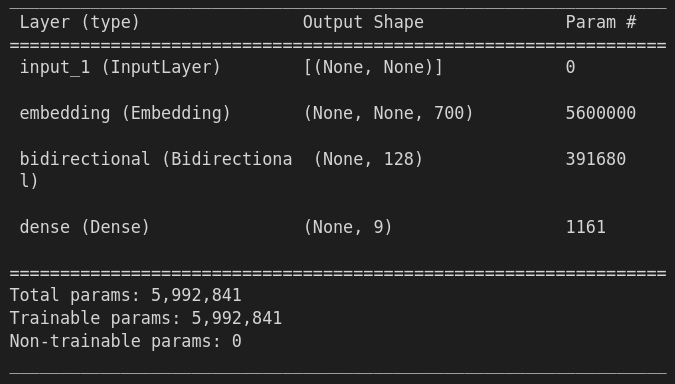
\includegraphics[scale=.3]{img/architecture_bilstm.png}
    \caption{Architecture du réseau BILSTM}
    \label{architecture_bilstm}
\end{figure}